%% v3.0 [2015/11/14]
%\documentclass[Proof,technicalreport]{ieicej}
\documentclass[technicalreport]{ieicej}
\usepackage[T1]{fontenc}
\usepackage{lmodern}
\usepackage{textcomp}
\usepackage{latexsym}
\usepackage{graphicx}
\usepackage[fleqn]{amsmath}
%\usepackage{amssymb}

\def\IEICEJcls{\texttt{ieicej.cls}}
\def\IEICEJver{3.0}
\newcommand{\AmSLaTeX}{%
 $\mathcal A$\lower.4ex\hbox{$\!\mathcal M\!$}$\mathcal S$-\LaTeX}
%\newcommand{\PS}{{\scshape Post\-Script}}
\def\BibTeX{{\rmfamily B\kern-.05em{\scshape i\kern-.025em b}\kern-.08em
 T\kern-.1667em\lower.7ex\hbox{E}\kern-.125em X}}

\jtitle{顔認識アルゴリズムを用いた擬似立体視の実現}
\jsubtitle{被写体の立体感をいかに作るか?}
%\etitle{How to Use \LaTeXe\ Class File (\IEICEJcls\ version \IEICEJver) 
        %for the Technical Report of the Institute of Electronics, Information 
        %and Communication Engineers}
%\esubtitle{Guide to the Technical Report and Template}

 \authorentry[hanako@denshi.ac.jp]{高松 真}{Makoto Takamatsu}{Tokyo}% 
\affiliate[Tokyo]{東京電機大学\hskip1zw
  〒120--8551 東京都足立区千住旭町}
 {Faculty of Engineering,
  First University\hskip1em
  Asahicho 5, Adachi-ku, Tokyo,
  120--8551 Japan}


\MailAddress{$\dagger$16ec068@ms.dendai.ac.jp}

\begin{document}
%\begin{jabstract}
%我々は擬似立体視という手法を用いることで,単眼写真の立体視を実現した.我々は相対深度に着目して擬似立体を実現している.
%しかし,我々はいままで,被写界深度の範囲を明確化せずに擬似立体視を作成した.そこで,今回は被写界深度の範囲とそれを超える部分との間を消失点検出を用いて定量的に測定可能にする。
%\end{jabstract}
\begin{jkeyword}
擬似立体視,相対深度,ハフ変換,被写界深度,ステレオマッチング
\end{jkeyword}

\maketitle

\section{まえがき}
単眼画像の立体視は困難な問題である.一枚の静止画像から立体視を実現する問題を解決する手段として,ハードウェアで実際の環境の深度を測定し,測定結果を単眼画像に加える方法[1]や深層学習が注目されている[2,3].我々は,ハードウェアを使用せず,ソフトウェアのみで単眼画像の擬似立体視を実現するために,物体認識アルゴリズムを用いて被写体を認識,被写体の顔サイズから相対深度を推定し,各被写体の深度を割り当て擬似立体視を実現する方法について検討した[].\\

我々の今までの研究では,地面の深度がすべての領域で等しく,反対に、各被写体の相対深度が異なるため,作成した擬似立体視を見ると被写体が地面から浮かんで見えるなどの違和感を感じることがあった.そこで本報告書で,立体的な見え方を実現するために筆者らは3点解決策を提案する.

1つ目は,ハフ変換を用いて被写界深度の範囲を定量的に測定する.つまり、被写界深度の範囲とそれを超える部分との間を消失点検出を用いて区別する。被写界深度とは、ピントを合わせた部分の前後のピントがあっているように見える範囲のことである。


%空は無限遠点に存在する領域であり,相対深度で扱うことは不可能な領域である.したがって,無限遠点である空の領域と相対深度として扱える被写体領域を区別するための消失線推定を行うことを提案する.

2つ目は,画像の下端から消失点まで地面の深度を変化させる。これは擬似立体視の見え方への違和感を減らすためである.その際、地面の深度グラデーションのかけ方について、線形と非線形で比較を行う。(現在、地面への深度グラデーションは非線形で行う方法はプログラムが完成している)

3つ目は、アナグリフ画像を作成した際に見られる黒い縁取り部分をなくす作業である。黒い部分を無くしてより自然な立体感を生み出すためBlure textureという手法を行う。Blure textureは、動く物体にBlure(ボケ)のかかったテクスチャをマッピングする技術である。シルエットが鮮明でテクスチャのつなぎ目が目立つときに使われる手法である[8][9][10][11]。

本報告書の構成を次に説明する。第2章が我々の従来法、第3章が消失点検出(ハフ変換)、第4章は地面の深度グラデーション、第5章はBlure Textureについて説明する。
%地平線の位置を推定することにより
\section{我々の従来法}
\subsection{顔認識}
\begin{figure}[t]
\begin{center}
\includegraphics[width=5cm,bb=0 0 570 428]{fig1.png}
\caption{顔認識}
\label{fig:1}
\end{center}
\end{figure}
顔認識アルゴリズムであるBiola-Jonesアルゴリズムを用いて1枚の人物集合写真から顔を認識,検出した顔のサイズを正方形のバインディングボックスで囲む.図\ref{fig:1}は顔のバインディングボックスで囲んである図である.

\subsection{相対深度算出}
被写体$i$の深度を以下の式:\begin{equation}D_i=\frac{255S_0}{S_i}\end{equation}で表す.ただし,$S_0$は最も後ろの被写体の顔サイズを,$S_i$は任意の被写体の顔サイズを表す.
\begin{figure}[t]
\begin{center}
\includegraphics[width=5cm,bb=0 0 4608 3456]{depth.jpg}
\caption{深度画像}
\label{fig:2}
\end{center}
\end{figure}

\subsection{擬似立体視作成}
各被写体の深度を使い,被写体を左右に移動させステレオビジョンを作成するために,移動量を算出する.移動量を以下の式:\begin{equation}P_i=M(1-\frac{D_i}{255})\end{equation}で表す.作成したステレオビジョンにアナグリフ処理を行う.図\ref{fig:4}は作成したアナグリフ画像である.
\begin{figure}[t]
\begin{center}
\includegraphics[width=5cm,bb=0 0 1116 418]{fig2.png}
\caption{ステレオビジョン作成}
\ref{fig:3}
\end{center}
\end{figure}

\begin{figure}[t]
\begin{center}
\includegraphics[width=5cm,bb=0 0 738 550]{fig3.png}
\caption{アナグリフ画像}
\label{fig:4}
\end{center}
\end{figure}

\section{消失点検出}
今までの私たちの研究では,最も後ろの被写体深度を255とし、最も後ろの被写体と背景に深度値255を適用した.したがって,実際には大きく距離が離れている背景と最も後ろの被写体を同じ深度で扱い擬似立体視を実現した.現在は、被写界深度の上部とそれを超える部分との境界をハフ変換を用いて消失線検出する.
ハフ変換とは以下の式\begin{equation}\hat \rho=x \cos \hat \theta +y \sin \hat \theta \end{equation}で表される.$\hat \rho$は,原点から直線までの符号付き距離,$\hat \theta$は原点から直線への垂線である.

式(1)は$xy$画像空間中の点を$\rho$ $\theta$パラメータ空間に写像すると点の数だけ直線を描くことができ,これらの直線は$\rho$ $\theta$パラメータ空間の1点$(\hat \rho,\hat \theta)$で交差することを示し,この交差する1点の座標を検出すれば$xy$画像空間中の直線を検出できる.画像空間中の直線を検出している様子が図\ref{fig5}である。


$\rho$ $\theta$パラメータ空間中の平行線は画像面上では一点で交わる.この1点を消失点と呼ぶ[4].
%ここに図を挿入!!

図\ref{fig6}の赤線はハフ変換によって得られた消失線である.
\begin{figure}[t]
\begin{center}
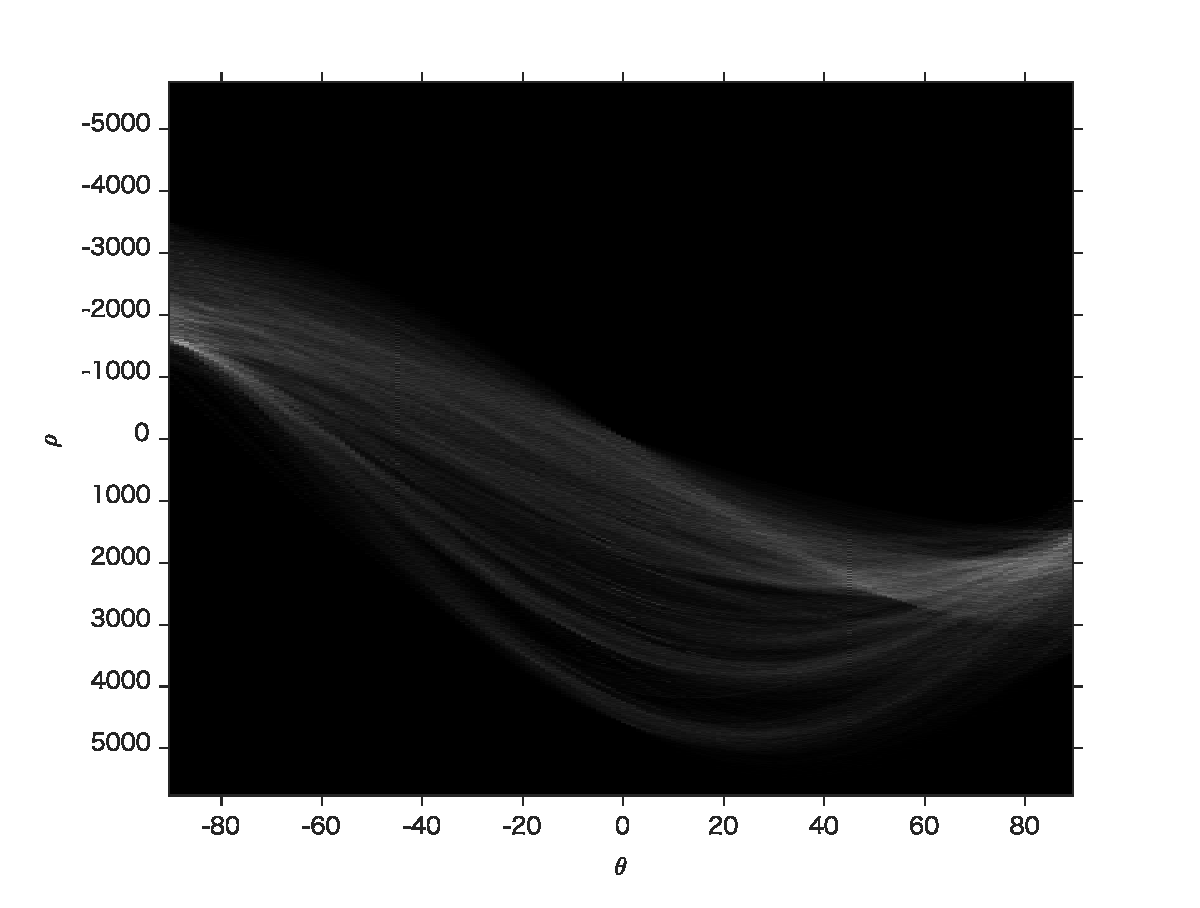
\includegraphics[width=7cm,clip]{hough.eps}
\caption{}
\label{fig5}
\end{center}
\end{figure}

\begin{figure}[t]
\begin{center}
\includegraphics[width=10cm, bb=0 0 1151 863]{fig4.png}
\caption{消失線検出}
\label{fig6}
\end{center}
\end{figure}


\section{地面領域の深度グラデーション}
\subsection{線形バージョン}
ハフ変換を用いて消失点を検出した.この消失点より上の領域を深度255とし,画像下端から消失点にかけて深度を線形にかける.
\subsection{非線形バージョン}
線形バージョンと同様にハフ変換を用いて、消失点を検出する。画像下端から消失点まで深度グラデーションをかける。消失点より上は255である。画像は消失点に近くなるにつれて急峻になることを踏まえて画像の深度を非線形でかける.$\log{x}$は収束するまでの距離が長いため、消失点に近くなると現れる急峻さを表現できない。そこで、$\log{x}$よりも収束速度がはやい$\sqrt{x}$を用いる。
\section{Blure texture}




%\bibliographystyle{sieicej}
%\bibliography{myrefs}
\begin{thebibliography}{99}% 文献数が10未満の時 {9}
\bibitem{1}{Julien N.P.Martel ,"An active Approach to Solving the Streo Matching Problem using Event-Based Sensors." 2018.}
\bibitem{2}{E.Shelaharmer,J.Long and T.Darrel"Fully Convolutional Networks for Semantic Segmentation."CVPR 2015.}
\bibitem{3}{Y.Luo "Single View Streo Matching."2018}
\bibitem{4}{画像情報教育振興協会:ディジタル画像処理,pp.238-243(2015)}
\bibitem{5}{A.Saxena and J.Schulte,Andrew Y.Ng ,"Depth Estimation using Monocular and Stereo Cues," IJCAI.2007.}
\bibitem{6}{J.Sun,H.Shum ,and N.Zheng,"Streo Matching Using Belief Propagation." }
\bibitem{7}{Z.Liu,X.Li ,and P.Luo,"Deep Learning Markov Random Field for Semantic Segmentation."2017.}
\bibitem{8}{Z.Wu,"Deep Markov Random Field for Image Modeling."2015}
\bibitem{9}{Morgan McGuire,and Padraic Hennessy,Michael Bukowski,Brian Osman,“A Reconstruction Filter for Plausible Motion Blur.”i3D(2012)}
\bibitem{10}{Jean-Philippe Guertin,and Morgan McGuire,Derek Nowrouzezahrai,“A Fast and Stable Feature-Aware Motion Blur Filter.”HPG '14 Proceedings of High Performance Graphics(2014)}
\bibitem{11}{Xuejiao Luo ,and Nestor Z. Salamon, Elmar Eisemann ,“Adding Motion Blur to Still Images.” Graphics Interface Conferenhce (2018)}


\end{thebibliography}

%\appendix


\end{document}
